\chapter{Grundlagen}

\section{Maschinelles Lernen (Machine Learning)}

\section{Physikalische Grundlagen zur Netzaktivität} \label{physikalischeGrundlagen}

\section{Erhebung der Messdaten}

    Um aussagekräftige Analysen und Klassifikationen über ein Stromnetz bzw. die Geräte in einem Stromnetz mit Maschinellem Lernen machen zu können, werden viele Trainings- und Testdaten benötigt.
    Die Daten bestehen aus verschiedenen physikalische Größen, die zu einem bestimmten Zeitpunkt in einem Stromnetz auftreten.
    Zu diesen Größen gehört die allgemeine Netzspannung, die Netzfrequenz sowie sieben harmonischen Oberwellen (vgl. \ref{physikalischeGrundlagen}).
    Um einen allgemeinen Überblick über den Verlauf der Netzaktivität zu erhalten sowie verschiedene Zeiten und Geräte vergleichen zu können, müssen Daten über lange Zeiträume erhoben werden.\\
    \newline
    Zur Erhebung der Werte zur Netzaktivität wurde ein WeSense-Messgerät\footnote{http://www.wesense-app.com/home-en/} verwendet.
    Dieses Gerät misst alle benötigten Werte und sendet diese über einen MQTT-Broker an einen Service von WeSense, welcher dann die Daten aufbereitet und in einer MSSQL Datenbank abspeichert.
    Die Werte werden sekündlich gemessen und in die Datenbank gespeichert, weshalb zunächst in eine row-based Datenbank gespeichert wird und später dann die Daten in eine column-based Datenbank zur schnellen Abfrage überführt werden.
    \newline

    Architektur Bild!!

    \subsection{Klassifikation der Messdaten}
        
        Durch die oben beschriebene Erhebung sind die physikalischen Werte zu bestimmten Zeitpunkten bestimmt worden.
        Zusätzlich wird nun zur Identifikation der Geräte sowie zum Maschinellen Lernen, genau definierte Zeiträume benötigt in denen bestimmte Geräte aktiv waren.
        Dies bedeutet, dass jedem Zeitpunkt ein oder mehrere Geräte zugewiesen werden. \\
        \newline
        Um diese gelabelten Daten zu erheben gibt es verschiedene Möglichkeiten.
        Die Daten können entweder durch eine Person, welche Zeiten zu denen sicher Geräte aktiv waren manuell erfasst, oder durch eine Maschine automatisch erhoben werden.
        Jedoch wird zur automatischen Erhebung ein weiteres Gerät benötigt, welches zwischen dem zu messenden Gerät und dem Stromnetz zwischengeschalten wird und sobald Strom fließt Daten erfasst.
        Somit werden die manuell durch eine Person erfasst.\\
        \newline
        Hierzu wurde eine progressive Web-App(vgl. Abbildung \ref{fig:WebApp1}) mit einer einfachen MySQL-Datenbank erstellt, mit der die Daten sehr einfach erfasst und abgespeichert werden können.

        \begin{figure}[h]
            \centering
            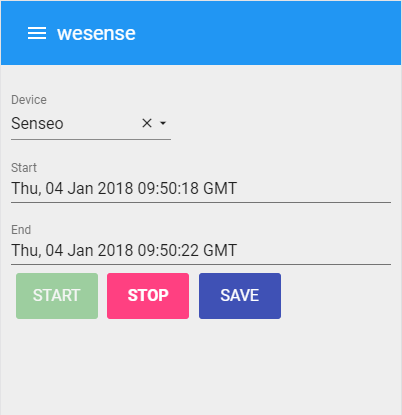
\includegraphics[width=0.5\textwidth]{WesenseConveyWebApp}
            \caption{Screenshot der progressive Web-App}
            \label{fig:WebApp1}
        \end{figure}
        